\documentclass{beamer}

\mode<presentation>
{
  \usetheme{Madrid}
  \usecolortheme{default}
  \usefonttheme{serif}
  \setbeamertemplate{navigation symbols}{}
  \setbeamertemplate{caption}[numbered]
} 

\usepackage[english]{babel}
\usepackage[utf8x]{inputenc}

\title[]{Macro Attention Indices for Stock Return Predictability}
\author[Arauz, Geiser, Stavropoulos, Tang]{Aaron Arauz Baumender  \\ Michael Adrian Geiser Pasquel \\ Andreas Stavropoulos \\ Zhiyi Tang}
\date{December 2023}

\begin{document}

\begin{frame}
  \titlepage
\end{frame}

\begin{frame}{Abstract}
  We conduct forecasts for equity risk premia utilizing linear and neural network models trained on sets of macroeconomic factors and macroeconomic attention indices. The macroeconomic factors set comprises the 14 features recommended in previous works by Goyal and Welch (2008). The set of macro attention indices includes the eight features constructed by Fisher et al. (2022). Equity risk premia represent the annualized excess return of the one-month S\&P 500 index over the prevailing risk-free rate, approximated by the yield on short-term Treasury Bills. Our analysis focuses on the period between 1985 and 2018, given the availability of the data. However, our results deviate from previous research, suggesting the need for further investigation into the datasets.
  \vspace{1em}

  \textbf{Keywords:} Equity risk premia; Macroeconomic factors; Macro economic attention indices; Neural networks; Financial forecast
\end{frame}

\begin{frame}{Outline}
  \tableofcontents
\end{frame}

\section{Introduction}
\begin{frame}{Introduction}
  \begin{itemize}
    \item \textbf{Background}
      \begin{itemize}
        \item Traditional focus on macroeconomic factors (MEF).
        \item Behavioral finance introduces macro attention indices (MAI) reflecting market sensitivity to information.
        \item Study recognizes interplay between MEF and MAI, and aims to contribute predictive models using linear and neural networks.
      \end{itemize}    
    \item \textbf{Objectives}
      \begin{itemize}
        \item Assess S\&P 500 (GSPC) Equity Risk Premia (ERP) predictive capacity of MEF and MEF using linear regression and neural networks.
      \end{itemize}     
    \item \textbf{Significance of the Study}
      \begin{itemize}
        \item Goes beyond traditional forecasting methods.
        \item Comprehensive analysis with linear and neural network models.
        \item Aims to inform investors, policymakers, and researchers, as well as to enhance understanding of equity market dynamics. 
      \end{itemize}
  \end{itemize}
\end{frame}

\section{Literature Review}
\begin{frame}{Literature Review}
  \begin{itemize}
    \item \textbf{Macroeconomic Factors}
      \begin{itemize}
        \item Insights from Fama and French (1988) and Goyal and Welch (2003) reveal importance of dividends and book value in ERP forecasting.
        \item Recent studies (Lo and Singh, 2003; Gu et al, 2019) use advanced techniques, revealing non linear dynamics.
      \end{itemize}
    \item \textbf{Macro Attention Indices}
      \begin{itemize}
        \item Studies by Andrei and Hasler (2006) and Nikkien et al. (2006) highlight the role in shaping investor sentiment.
        \item Recent research (Ma et al., 2022) emphasizes improved predictive accuracy during market uncertainty.
      \end{itemize}
    \item \textbf{Comparison of Factors and Indices}
      \begin{itemize}
        \item No existing deep comparison of models models, which may offer a more robust framework.
        \item Study uses linear regression models and neural networks for a comprehensive analysis.
      \end{itemize}
  \end{itemize}
\end{frame}

\section{Theoretical Framework}
\begin{frame}{Theoretical Framework}
  \begin{itemize}
    \item \textbf{Market Dynamics Beyond Efficiency}
      \begin{itemize}
        \item Challenges traditional Efficient Market Hypothesis.
        \item Acknowledges anomalies and deviations from efficiency, especially during heightened investor attention.
        \item Highlights the need for alternative frameworks beyond complete market efficiency.
      \end{itemize}
    \item \textbf{Behavioral Finance and Investor Attention}
      \begin{itemize}
        \item Integrates behavioral finance insights into decision-making.
        \item Considers investor attention and herd behavior, leading to overreaction or underreaction.
        \item Accounts for sentiment and attention in forecasting models, recognizing limitations of purely rational assumptions.
      \end{itemize}
    \item \textbf{Neural Networks in Financial Forecasting}
      \begin{itemize}
        \item Utilizes neural networks to capture complex relationships.
        \item Addresses limitations of traditional linear models.
        \item Enhances modeling of interactions between MEF and MAI impacting ERP.
      \end{itemize}  
  \end{itemize}
\end{frame}

\begin{frame}{Theoretical Framework (continued)}
  \begin{itemize}
    \item \textbf{Model Specification}
    \newline
      \begin{itemize}
        \item \textbf{MEF:} Log Dividend-Price $\|$ Log Dividend Yield $\|$ Log Earnings-Price $\|$ Log Dividend-Payout $\|$ Equity Premium Vol $\|$ Book-to-Market Ratio $\|$ Net Equity Expansion $\|$ Treasury Bill Rate $\|$ Long-Term Yield $\|$ Long-Term Return $\|$ Term Spread $\|$ Default Yield Spread $\|$ Default Return Spread $\|$ Inflation
        \newline
        \item \textbf{MAI:} Credit Rating $\|$ Gross Domestic Product $\|$ House Market $\|$ Inflation $\|$ Monetary $\|$ Oil $\|$ Unemployment Rate $\|$ US Dollar
        \newline
        \item \textbf{ERP:} GSPC Equity Risk Premia
      \end{itemize}
  \end{itemize}
\end{frame}

\section{Methodology}
\begin{frame}{Methodology}
  \begin{itemize}
    \item \textbf{Data Management}
    Historical data from 1.1.1985 to 31.12.2018, daily, monthly, and quarterly frequencies. Collected from various repositories, organized chronologically for model training.
      \begin{itemize}
        \item \textbf{Data Collection (Raw Data):} MEF and MAI data collected from specific GitHub repositories. GSPC data collected from Yahoo Finance.
        \item \textbf{Data Cleaning (Interim Data):} Preprocessing steps applied to address missing values in MAI raw databases.
        \item \textbf{Data Processing (Processed Data):} MEF and MAI data undergo processing to construct data for model training. Calculations include transformations and interpolations to derive key macroeconomic factors and attention indexes.
      \end{itemize}
  \end{itemize}
\end{frame}

\begin{frame}{Methodology (continued)}
  \begin{itemize}
    \item \textbf{Data Selection}
    \begin{itemize}
        \item Utilizing the \href{https://baumender11.shinyapps.io/Alpha/}{Interactive Shiny App} facilitates visualization of the impact of various features and temporal ranges.
        \item Flexibility to:
        \begin{itemize}
            \item select any subset of the 14 MEF variables,
            \item select any subset of the 8 MAI variables,
            \item select any time window ranging from 1.1.1985 to 31.12.2018,
            \item select different temporal frequencies of the data (daily, monthly, quarterly).
        \end{itemize}
        \item The MEF model results are denoted by blue lines, the MAI model results by green lines, and the veritable values by the red line.
        \item In the next slides we provide a few cases.
    \end{itemize}
  \end{itemize}
\end{frame}

\begin{frame}{Methodology (continued)}
  \begin{itemize}
    \item Quarterly data between 1.1.1985 and 31.12.2018 of MEF Log Dividend-Price (solid blue), MEF Log Dividend Yield (dashed blue), MAI Credit Rating (dashed green), and MKT GSPC (solid red) are selected.
  \end{itemize}
    \begin{figure}[H]
        \centering
        \begin{minipage}{.80\textwidth}
            \centering
            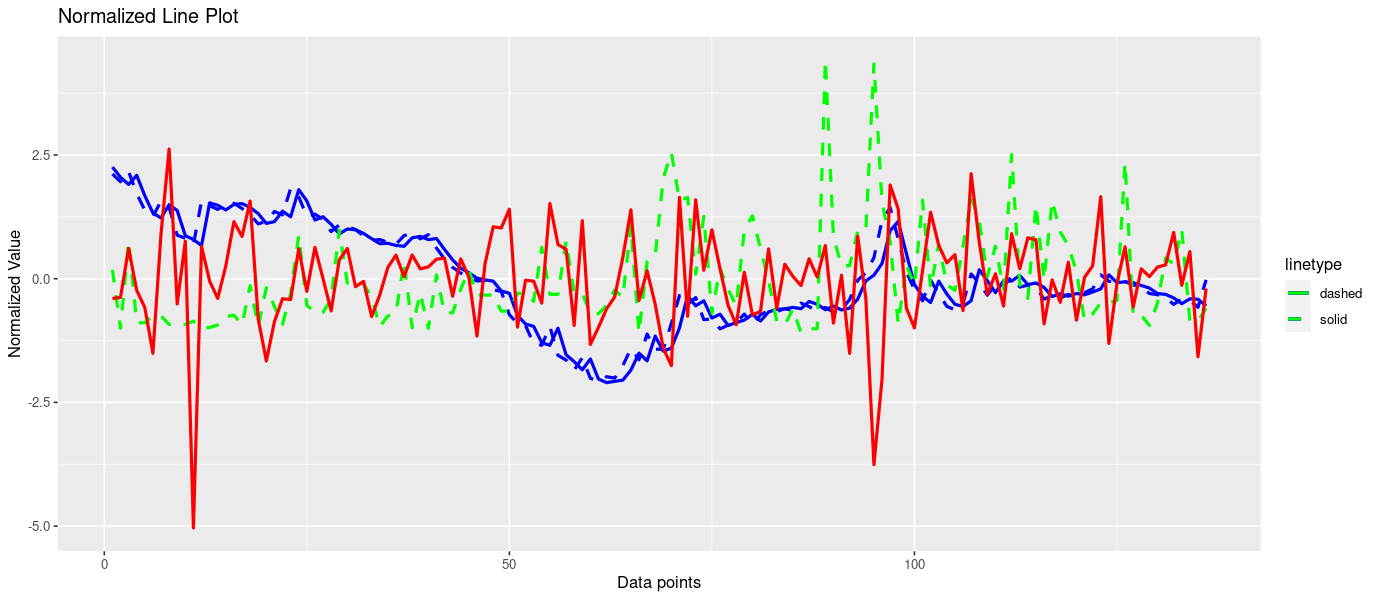
\includegraphics[width=\linewidth]{MEF_dpdy_MAI_cr.png}
            \caption{Shiny app variable selection outcome, Case 1.- \href{https://baumender11.shinyapps.io/Alpha/}{Interactive Shiny App}}
            \label{fig:linear_prediction}
        \end{minipage}
    \end{figure}
\end{frame}

\begin{frame}{Methodology (continued)}
  \begin{itemize}
    \item Quarterly data between 1.1.1985 and 31.12.2018 of MEF Log Dividend-Price (solid blue), MEF Log Dividend Yield (dotted blue), MEF Log Earnings-Price (dashed blue), MAI Credit Rating (dotted green), MAI Gross Domestic Product (solid green), and MKT GSCP (solid red) are selected.
  \end{itemize}
    \begin{figure}[H]
        \centering
        \begin{minipage}{.80\textwidth}
            \centering
            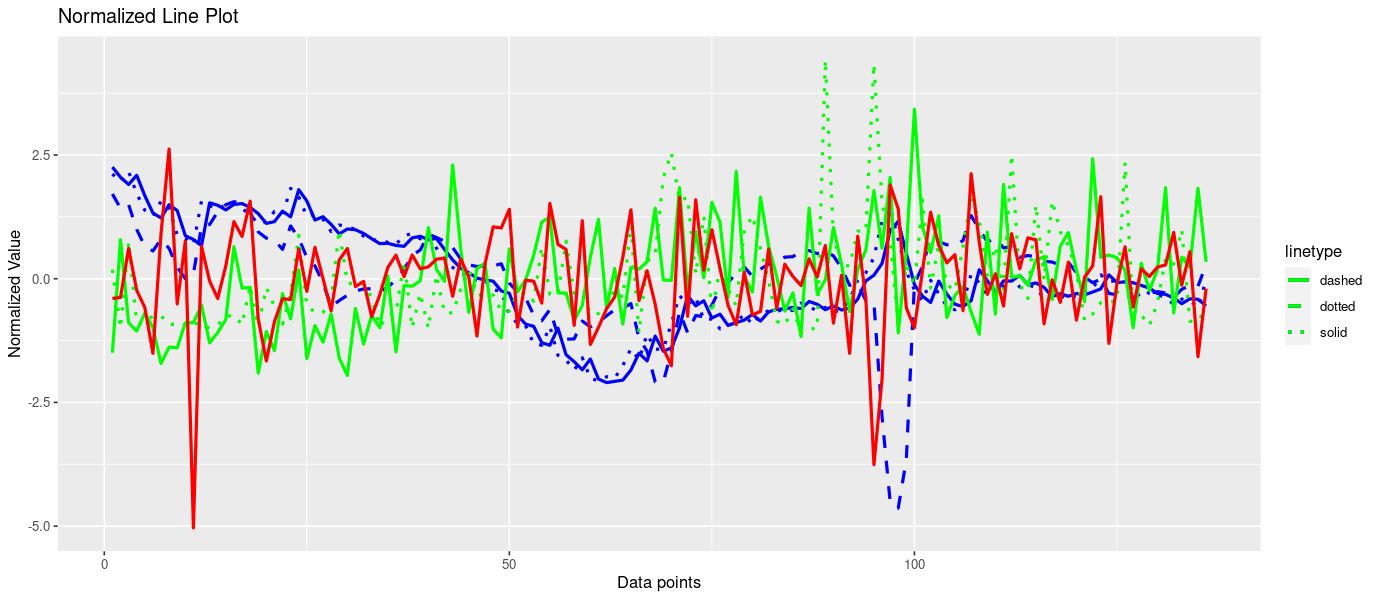
\includegraphics[width=\linewidth]{MEF_dpdyep_MAI_crgdp.png}
            \caption{Shiny app variable selection outcome, Case 2.- \href{https://baumender11.shinyapps.io/Alpha/}{Interactive Shiny App}}
            \label{fig:linear_prediction}
        \end{minipage}
    \end{figure}
\end{frame}

\begin{frame}{Methodology (continued)}
  \begin{itemize}
    \item{ Correlation heatmaps, MEF data between, 1.1.1985 and 31.12.2018.} 
  \end{itemize}

  \begin{figure}[H]
    \centering
    \begin{minipage}{0.32\textwidth}
      \centering
      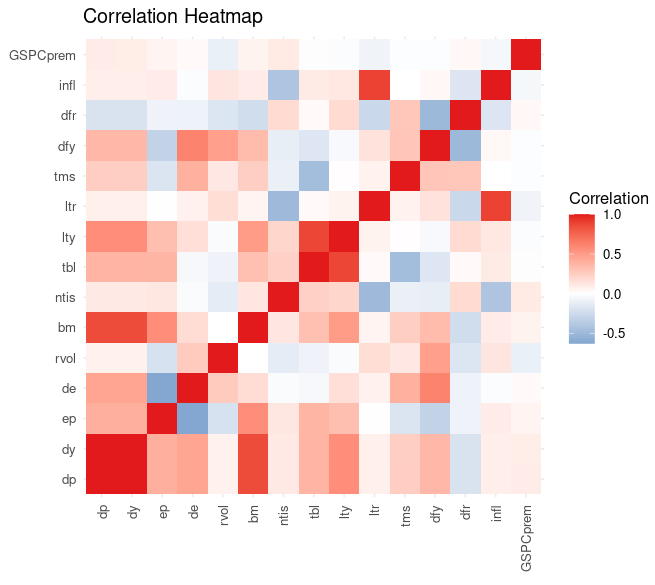
\includegraphics[width=\linewidth]{Cormap_MEF_Daily_85.png}
      \caption{MEF daily.}
      \label{fig:linear_prediction}
    \end{minipage}\hfill
    \begin{minipage}{0.32\textwidth}
      \centering
      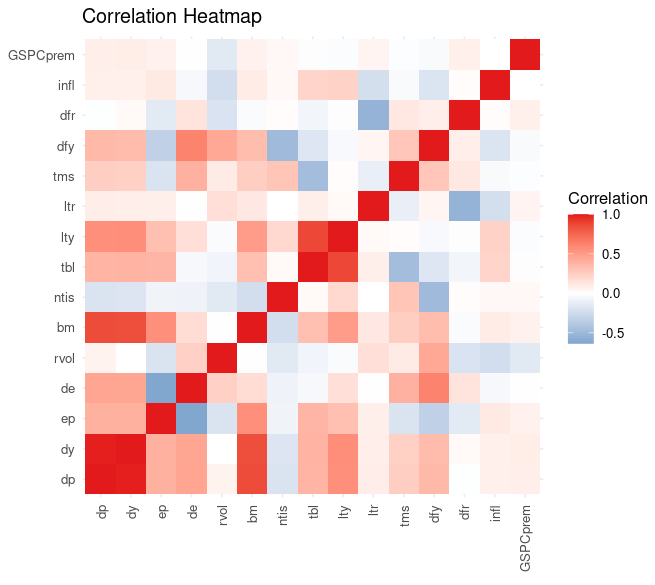
\includegraphics[width=\linewidth]{Cormap_MEF_Monthly_85.png}
      \caption{MEF monthly.}
      \label{fig:nn_prediction}
    \end{minipage}\hfill
    \begin{minipage}{0.32\textwidth}
      \centering
      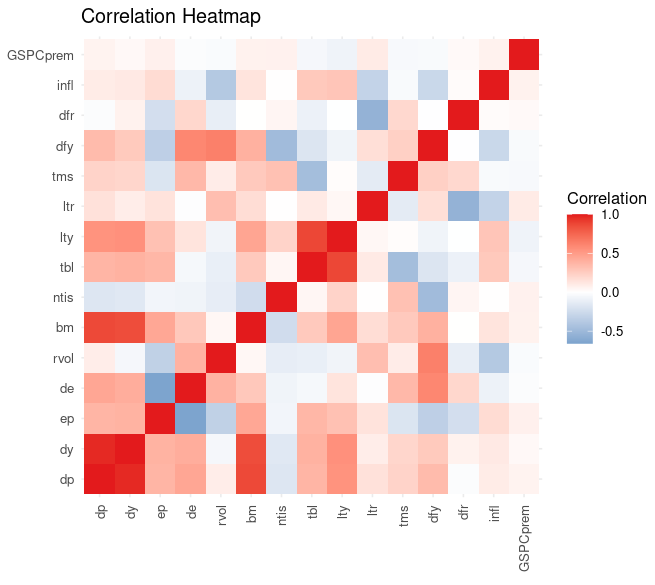
\includegraphics[width=\linewidth]{Cormap_MEF_Quarterly_85.png} 
      \caption{MEF quarterly.}
      \label{fig:third_prediction}
    \end{minipage}
  \end{figure}
\end{frame}

\begin{frame}{Methodology (continued)}
  \begin{itemize}
    \item{ Correlation heatmaps, MEF data between, 1.1.2000 and 31.12.2018}
  \end{itemize}
  \begin{figure}[H]
    \centering
    \begin{minipage}{0.32\textwidth}
      \centering
      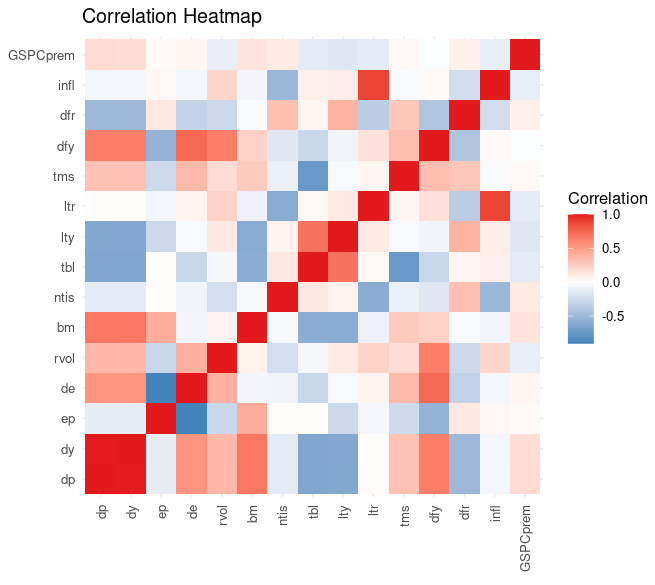
\includegraphics[width=\linewidth]{Cormap_MEF_Daily_00.png}
      \caption{MEF daily.}
      \label{fig:linear_prediction}
    \end{minipage}\hfill
    \begin{minipage}{0.32\textwidth}
      \centering
      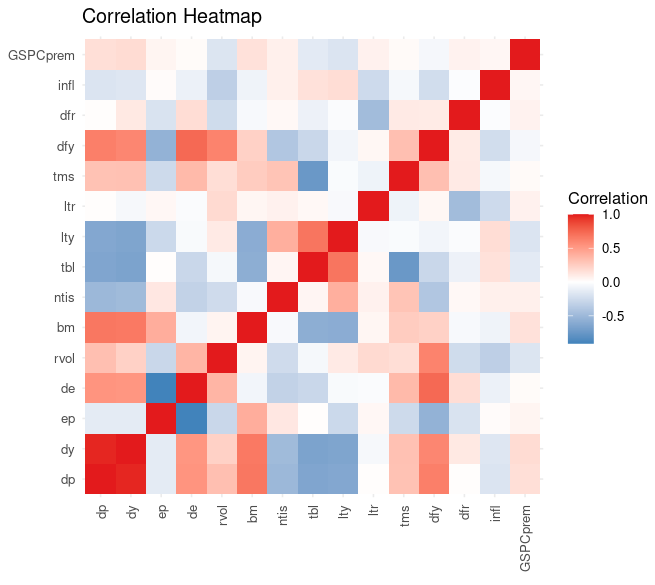
\includegraphics[width=\linewidth]{Cormap_MEF_Monthly_00.png}
      \caption{MEF monthly.}
      \label{fig:nn_prediction}
    \end{minipage}\hfill
    \begin{minipage}{0.32\textwidth}
      \centering
      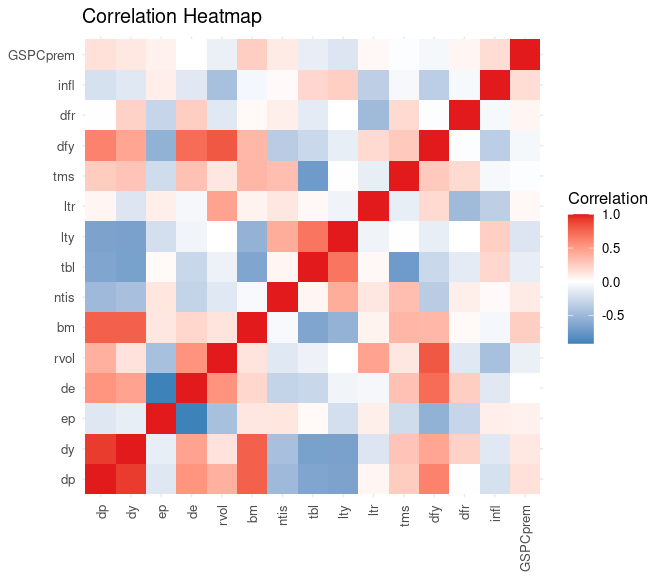
\includegraphics[width=\linewidth]{Cormap_MEF_Quarterly_00.png} 
      \caption{MEF quarterly.}
      \label{fig:third_prediction}
    \end{minipage}
  \end{figure}
\end{frame}

\begin{frame}{Methodology (continued)}
  \begin{itemize}
    \item \textbf{Model Training}
      \begin{itemize}
        \item Two approaches: Ridge regression and neural network models.
        \item Linear regression uses the standard equation with gradient descent and Ridge regularization.
        \item Neural network employs traditional feedforward architecture.
        \item Root Mean Squared Error (RMSE) used to assess performance.
      \end{itemize}
    \item \textbf{Comparison and Interpretation}
      \begin{itemize}
        \item Comparative analysis of results from both models.
        \item Evaluation based on RMSE for different combinations of economic data (MAI and MEF) and target variable (1-month GSPC ERP).
        \item Daily and monthly frequencies considered.
      \end{itemize}
  \end{itemize}
\end{frame}

\section{Empirical Analysis}
\begin{frame}{Empirical Analysis}
  \begin{itemize}
    \item \textbf{Data Overview}
    \begin{itemize}
      \item We used six datasets with their characteristics summarized in the following table:
    \end{itemize}
  \end{itemize}

  \begin{table}[H]
    \centering
    \resizebox{\textwidth}{!}{%
      \begin{tabular}{|c|c|c|c|c|}
        \hline
        \textbf{Dataset} & \textbf{\# of Variables} & \textbf{Frequency} & \textbf{Time Period} & \textbf{\# of Samples} \\ \hline
        MEF Daily & 14 & Daily & 1985/01/02-2018/12/31 & 8523 \\ \hline
        MAI Daily & 8 & Daily & 1985/01/02-2018/12/31 & 8523 \\ \hline
        MKT Daily & 1 & Daily & 1985/01/02-2018/12/31 & 8523 \\ \hline
        MEF Monthly & 14 & Monthly & 1985/01/31-2018/12/31 & 408 \\ \hline
        MAI Monthly & 8 & Monthly & 1985/01/31-2018/12/31 & 408 \\ \hline
        MKT Monthly & 1 & Monthly & 1985/01/31-2018/12/31 & 408 \\ \hline
      \end{tabular}%
    }
    \caption{Description of Datasets used for model training.}
    \label{tab:Datasets}
  \end{table}
\end{frame}

\begin{frame}{Empirical Analysis (continued)}
  \begin{itemize}
    \item \textbf{Model Implementation: Ridge Regression Model}
      \begin{itemize}
        \item Implemented ridge regression using MEF and MAI data as independent variables.
        \item Trained on four datasets: MEF monthly, MAI monthly, MEF daily, MAI daily, establishing a linear relationship with GSPC data (MKT monthly, MKT daily).
        \item Specifications:
          \begin{itemize}
            \item K-fold cross-validation (5 folds) to tune hyperparameter.
            \item Grid of tested values: [\(10^{-5}\), \(10^{-4}\), \(10^{-3}\), \(10^{-2}\), \(10^{-1}\), 1, 10, \(10^2\), \(10^3\), \(10^4\), \(10^5\)].
            \item Train-test split: 80% - 20%.
          \end{itemize}
        \item Training approach:
          \begin{itemize}
            \item For monthly datasets (408 points), the model is trained 10 times with different splits, reporting average RMSE.
            \item For daily datasets, the model is trained once, and RMSE is reported.
          \end{itemize}
      \end{itemize}
  \end{itemize}
\end{frame}

\begin{frame}{Empirical Analysis (continued)}
  \begin{itemize}
    \item \textbf{Model Implementation: Neural Network Model}
      \begin{itemize}
        \item Implemented a feedforward architecture with the following specifications:
          \begin{itemize}
            \item Two hidden layers (64 and 32 neurons).
            \item Two dropout layers (30% and 50% dropping rate) following each hidden layer.
            \item Single neuron output.
            \item Adam optimizer with a learning rate of 0.01.
            \item Batch size: 32.
            \item Number of epochs: 10.
          \end{itemize}
        \item Training approach:
          \begin{itemize}
            \item For monthly data, the model is trained 10 times with different train-test splits, and the average RMSE is reported.
            \item For daily data, the model is trained and predicted once.
          \end{itemize}
        \item Note: Meaningful results weren't expected from monthly datasets (408 points) due to limited data for efficient neural network training. However, this approach is used as a reference and for comparison with the regression model.
      \end{itemize}
  \end{itemize}
\end{frame}

\begin{frame}{Empirical Analysis (continued)}
    \begin{itemize}
        \item \textbf{Results}
            \begin{itemize}
                \item The average root mean square error (RMSE) of eight different models (two types of models on four datasets) is tested on ten different random train-test splits of each dataset.
            \end{itemize}
    \end{itemize}

    \begin{table}[H]
        \centering
        \begin{tabular}{|c|c|c|}
          \hline
          \textbf{Model} & \textbf{Input Data} & \textbf{RMSE on Test Set} \\ \hline
          \multirow{Linear Model} & MEF Daily & 53.243 \\ \cline{2-3} 
          & MAI Daily & 54.677 \\ \cline{2-3} 
          & MEF Monthly & 54.307 \\ \cline{2-3} 
          & MAI Monthly & 53.571 \\ \hline
          \multirow{NN Model} & MEF Daily & 54.142 \\ \cline{2-3} 
          & MAI Daily & 54.063 \\ \cline{2-3} 
          & MEF Monthly & 52.717 \\ \cline{2-3} 
          & MAI Monthly & 53.096 \\ \hline
        \end{tabular}
        \caption{Comparison of RMSE of different models}
        \label{tab:PerformanceResults}
    \end{table}
\end{frame}

\begin{frame}{Empirical Analysis (continued)}
  \begin{figure}[H]
    \centering
    \begin{subfigure}{\textwidth}
      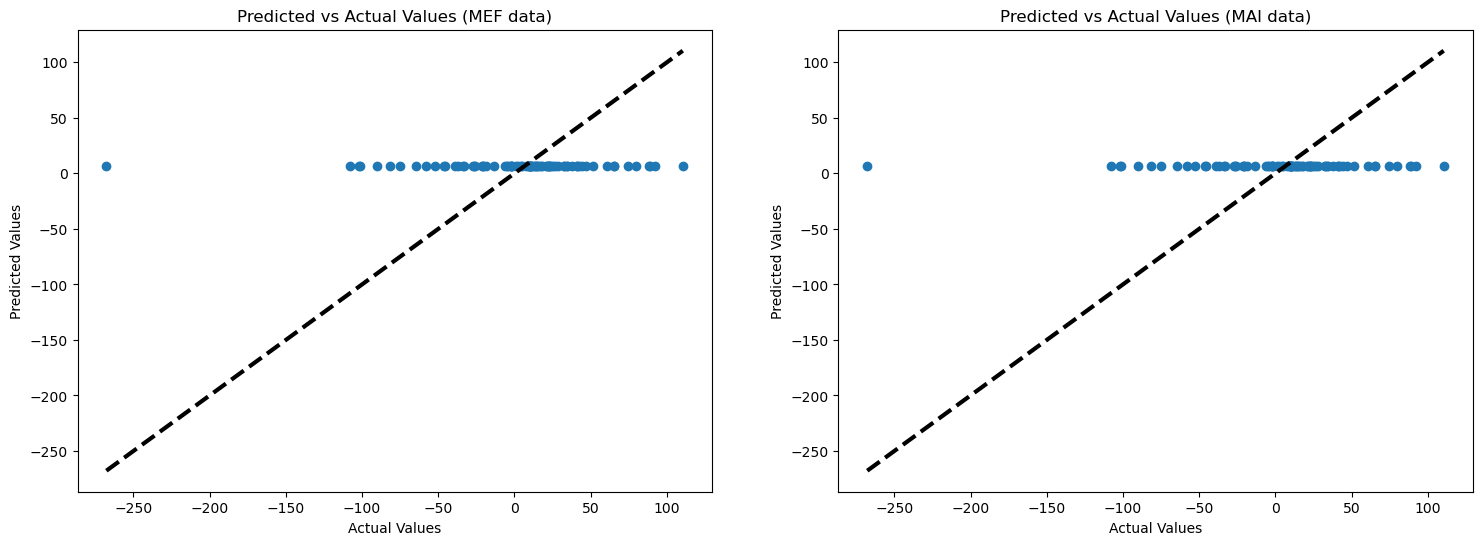
\includegraphics[width=.65\linewidth]{true_vs_pred_M_Regr.png}
      \caption{True vs Predicted values for monthly data (Regression)}
      \label{fig:monthly_regression}
    \end{subfigure}
    \begin{subfigure}{\textwidth}
      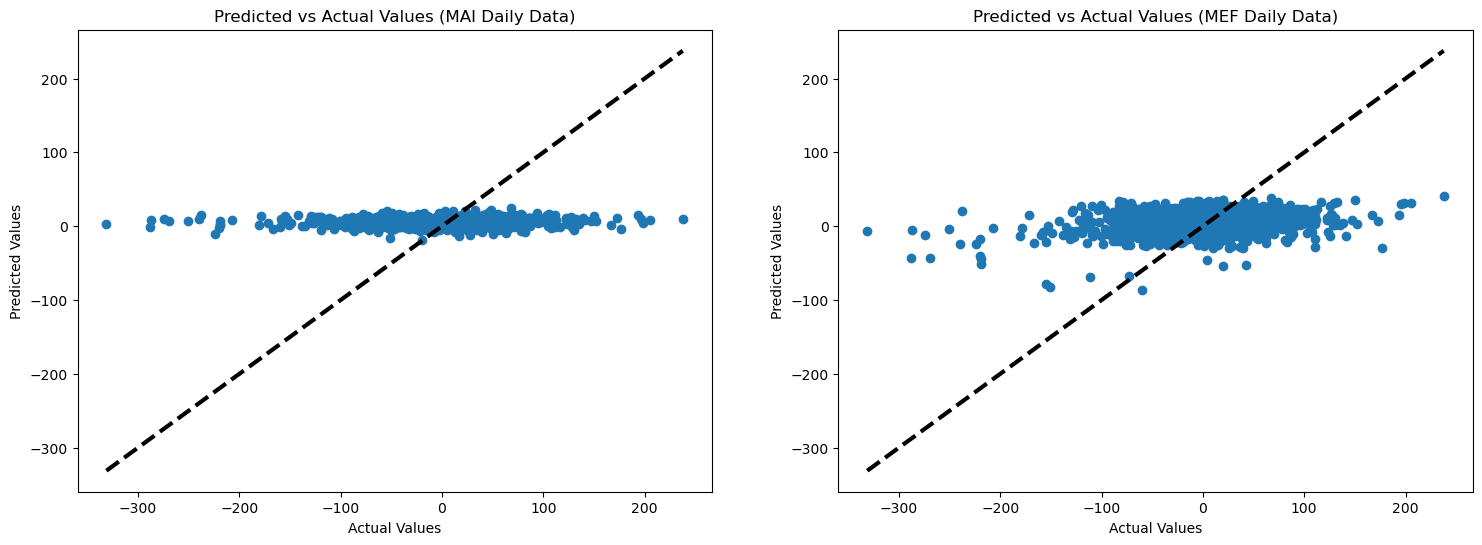
\includegraphics[width=.65\linewidth]{true_vs_pred_D_Regr.png}
      \caption{True vs Predicted values for daily data (Regression)}
      \label{fig:daily_regression}
    \end{subfigure}
  \end{figure}
\end{frame}

\begin{frame}{Empirical Analysis (continued)}
  \begin{figure}
    \centering
    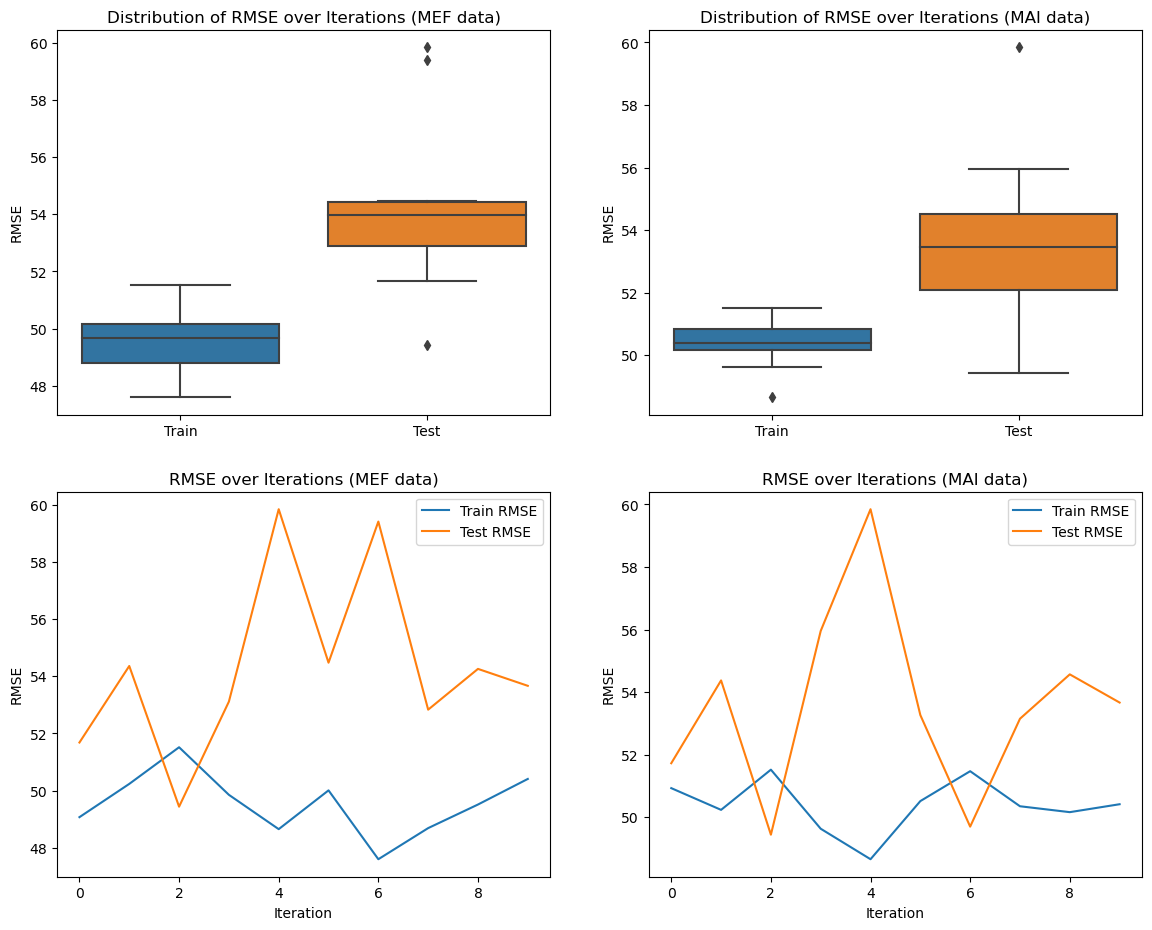
\includegraphics[width=0.70\textwidth]{Distribution of RMSE_Linear_M.png}
    \caption{Distribution of RMSE over iterations, linear models on monthly data.}
    \label{fig:linear_prediction_ii}
  \end{figure}
\end{frame}

\begin{frame}{Empirical Analysis (continued)}
  \begin{itemize}
    \item Distribution and boxplots of RMSE over iterations, Neural Networks
on monthly data
  \end{itemize}
  \begin{figure}[H]
    \centering
    \begin{minipage}{0.48\textwidth}
      \centering
      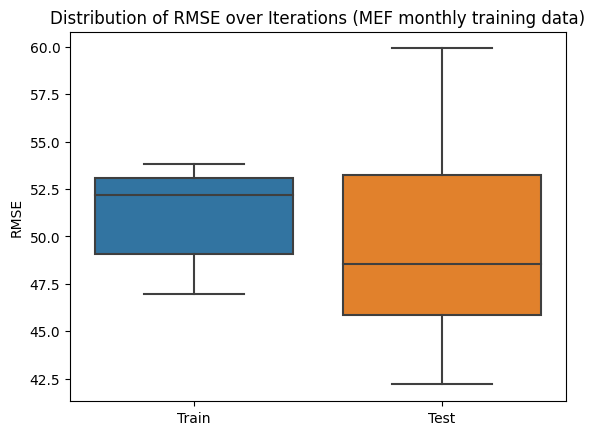
\includegraphics[width=\linewidth]{Distribution of RMSE_NN_MEF_M.png}
      \caption{MEF monthly.}
      \label{fig:linear_prediction}
    \end{minipage}\hfill
    \begin{minipage}{0.48\textwidth}
      \centering
      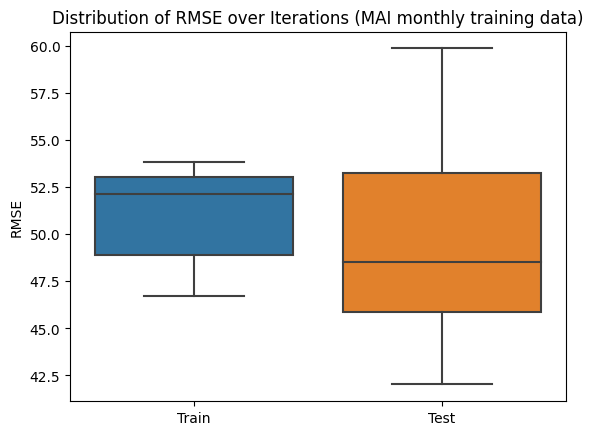
\includegraphics[width=\linewidth]{Distribution of RMSE_NN_MAI_M.png}
      \caption{MAI monthly.}
      \label{fig:nn_prediction}
    \end{minipage}
  \end{figure}
\end{frame}

\begin{frame}{Empirical Analysis (continued)}
  \begin{itemize}
    \item True vs Predicted values for daily data (Neural Network)
  \end{itemize}
  \begin{figure}[H]
    \centering
    \begin{minipage}{0.48\textwidth}
      \centering
      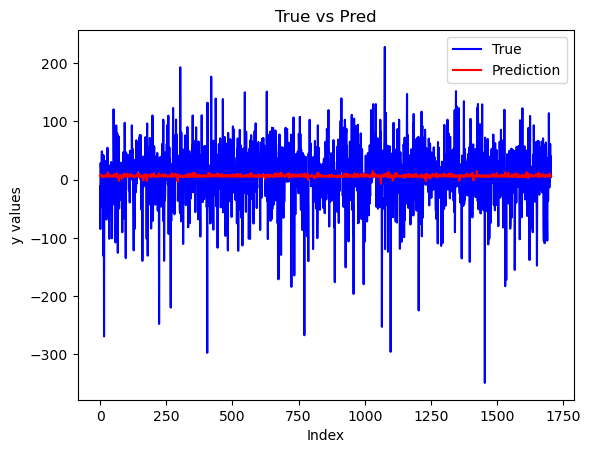
\includegraphics[width=\linewidth]{true_vs_pred_mai_D_NN.png}
      \caption{MEF daily.}
      \label{fig:linear_prediction}
    \end{minipage}\hfill
    \begin{minipage}{0.48\textwidth}
      \centering
      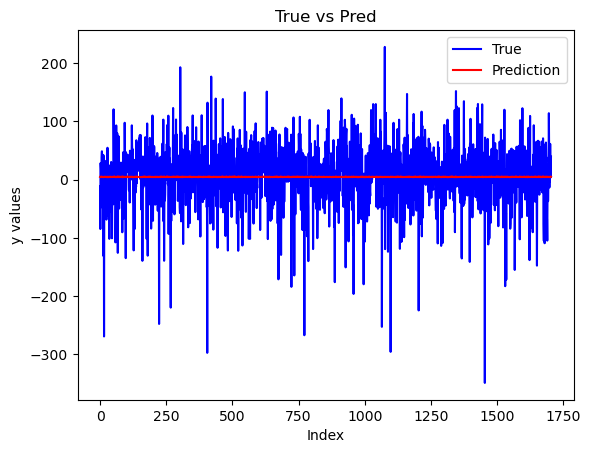
\includegraphics[width=\linewidth]{true_vs_pred_mef_D_NN.png}
      \caption{MAI daily.}
      \label{fig:nn_prediction}
    \end{minipage}
  \end{figure}
\end{frame}

\begin{frame}{Empirical Analysis (Continued)}
    \begin{itemize}
            \item \textbf{Model Selection}
            \begin{itemize}
                \item The inefficiency of both models (Ridge Regression, Neural Network) is evident in Table 2, highlighting their inability to predict the excess annualized returns of S\&P500.
                \item These results do not suggest a mere bad fit; rather, all models exhibit a lack of effective training and prediction within a narrow range.
                \item Given these findings, selecting a superior-performing model becomes challenging.
            \end{itemize}
    \end{itemize}
\end{frame}

\section{Discussion}
\begin{frame}{Discussion}
  \begin{itemize}
    \item \textbf{Summary} 
    \begin{itemize}
        \item Study aimed to forecast ERP using regression and neural network models, incorporating MEF and MAI datasets, targeting S\&P500 excess return.
        \item Despite utilizing data from 1985 to 2018, sourced from GitHub repositories and Yahoo Finance, predictive models showed significant deviations from established research.
    \end{itemize}
    \item \textbf{Interpretation of Results}
    \begin{itemize}
        \item Lack of predictive efficacy in MAI data contradicts literature.
        \item Limited usefulness of traditionally used MEF data in predicting stock returns (issues with data preprocessing, model complexity, or capturing relationships over a wide time frame).
        \item  Reasons for poor model performance include weak relationships between features and the target variable, inadequate data preprocessing, inappropriate hyperparameter tuning, insufficient model complexity (especially for neural networks), and non-stationarity of statistical properties in stock returns.
    \end{itemize}
  \end{itemize}
\end{frame}

\begin{frame}{Discussion (continued)}
  \begin{itemize}
    \item \textbf{Summary} 
    \begin{itemize}
        \item Experiment with combinations of MAI and MEF features as inputs to predictive models.
        \item Explore advanced preprocessing techniques, outlier detection methods, and strategies for handling missing data to enhance the quality of model inputs.
        \item Conduct a comprehensive hyperparameter search to optimize model performance.
        \item Explore more sophisticated modeling approaches beyond regression and neural networks.
        \item Consider focusing on shorter time ranges instead of the entire dataset or implement advanced time series analysis techniques to address non-stationarity.
    \end{itemize}
  \end{itemize}
\end{frame}

\section{References}
\begin{frame}{References}
  \begin{itemize}
    \item Fama and French (1988): \emph{Dividend Yields and Expected Stock Returns}
    \item Goyal and Welch (2003): \emph{Predicting the Equity Premium with Dividend Ratios}
    \item Lo and Singh (2003): \emph{Deep-learning models for forecasting financial risk premia and their interpretations}
    \item Gu, Kelly, and Xiu (2019): \emph{Empirical Asset Pricing via Machine Learning}
    \item Andrei and Hasler (2012): \emph{Investors’ Attention and Stock Market Volatility}
    \item Nikkinen, Omran, Sahlström, and Äijö (2006): \emph{Global stock market reactions to scheduled U.S. macroeconomic news announcements}
    \item Ma, Lu, Liu, and Huang (2022): \emph{Macroeconomic attention and stock market return predictability}
  \end{itemize}
\end{frame}

\end{document}
